\documentclass[1p]{elsarticle_modified}
%\bibliographystyle{elsarticle-num}

%\usepackage[colorlinks]{hyperref}
%\usepackage{abbrmath_seonhwa} %\Abb, \Ascr, \Acal ,\Abf, \Afrak
\usepackage{amsfonts}
\usepackage{amssymb}
\usepackage{amsmath}
\usepackage{amsthm}
\usepackage{scalefnt}
\usepackage{amsbsy}
\usepackage{kotex}
\usepackage{caption}
\usepackage{subfig}
\usepackage{color}
\usepackage{graphicx}
\usepackage{xcolor} %% white, black, red, green, blue, cyan, magenta, yellow
\usepackage{float}
\usepackage{setspace}
\usepackage{hyperref}

\usepackage{tikz}
\usetikzlibrary{arrows}

\usepackage{multirow}
\usepackage{array} % fixed length table
\usepackage{hhline}

%%%%%%%%%%%%%%%%%%%%%
\makeatletter
\renewcommand*\env@matrix[1][\arraystretch]{%
	\edef\arraystretch{#1}%
	\hskip -\arraycolsep
	\let\@ifnextchar\new@ifnextchar
	\array{*\c@MaxMatrixCols c}}
\makeatother %https://tex.stackexchange.com/questions/14071/how-can-i-increase-the-line-spacing-in-a-matrix
%%%%%%%%%%%%%%%

\usepackage[normalem]{ulem}

\newcommand{\msout}[1]{\ifmmode\text{\sout{\ensuremath{#1}}}\else\sout{#1}\fi}
%SOURCE: \msout is \stkout macro in https://tex.stackexchange.com/questions/20609/strikeout-in-math-mode

\newcommand{\cancel}[1]{
	\ifmmode
	{\color{red}\msout{#1}}
	\else
	{\color{red}\sout{#1}}
	\fi
}

\newcommand{\add}[1]{
	{\color{blue}\uwave{#1}}
}

\newcommand{\replace}[2]{
	\ifmmode
	{\color{red}\msout{#1}}{\color{blue}\uwave{#2}}
	\else
	{\color{red}\sout{#1}}{\color{blue}\uwave{#2}}
	\fi
}

\newcommand{\Sol}{\mathcal{S}} %segment
\newcommand{\D}{D} %diagram
\newcommand{\A}{\mathcal{A}} %arc


%%%%%%%%%%%%%%%%%%%%%%%%%%%%%5 test

\def\sl{\operatorname{\textup{SL}}(2,\Cbb)}
\def\psl{\operatorname{\textup{PSL}}(2,\Cbb)}
\def\quan{\mkern 1mu \triangleright \mkern 1mu}

\theoremstyle{definition}
\newtheorem{thm}{Theorem}[section]
\newtheorem{prop}[thm]{Proposition}
\newtheorem{lem}[thm]{Lemma}
\newtheorem{ques}[thm]{Question}
\newtheorem{cor}[thm]{Corollary}
\newtheorem{defn}[thm]{Definition}
\newtheorem{exam}[thm]{Example}
\newtheorem{rmk}[thm]{Remark}
\newtheorem{alg}[thm]{Algorithm}

\newcommand{\I}{\sqrt{-1}}
\begin{document}

%\begin{frontmatter}
%
%\title{Boundary parabolic representations of knots up to 8 crossings}
%
%%% Group authors per affiliation:
%\author{Yunhi Cho} 
%\address{Department of Mathematics, University of Seoul, Seoul, Korea}
%\ead{yhcho@uos.ac.kr}
%
%
%\author{Seonhwa Kim} %\fnref{s_kim}}
%\address{Center for Geometry and Physics, Institute for Basic Science, Pohang, 37673, Korea}
%\ead{ryeona17@ibs.re.kr}
%
%\author{Hyuk Kim}
%\address{Department of Mathematical Sciences, Seoul National University, Seoul 08826, Korea}
%\ead{hyukkim@snu.ac.kr}
%
%\author{Seokbeom Yoon}
%\address{Department of Mathematical Sciences, Seoul National University, Seoul, 08826,  Korea}
%\ead{sbyoon15@snu.ac.kr}
%
%\begin{abstract}
%We find all boundary parabolic representation of knots up to 8 crossings.
%
%\end{abstract}
%\begin{keyword}
%    \MSC[2010] 57M25 
%\end{keyword}
%
%\end{frontmatter}

%\linenumbers
%\tableofcontents
%
\newcommand\colored[1]{\textcolor{white}{\rule[-0.35ex]{0.8em}{1.4ex}}\kern-0.8em\color{red} #1}%
%\newcommand\colored[1]{\textcolor{white}{ #1}\kern-2.17ex	\textcolor{white}{ #1}\kern-1.81ex	\textcolor{white}{ #1}\kern-2.15ex\color{red}#1	}

{\Large $\underline{12a_{0756}~(K12a_{0756})}$}

\setlength{\tabcolsep}{10pt}
\renewcommand{\arraystretch}{1.6}
\vspace{1cm}\begin{tabular}{m{100pt}>{\centering\arraybackslash}m{274pt}}
\multirow{5}{120pt}{
	\centering
	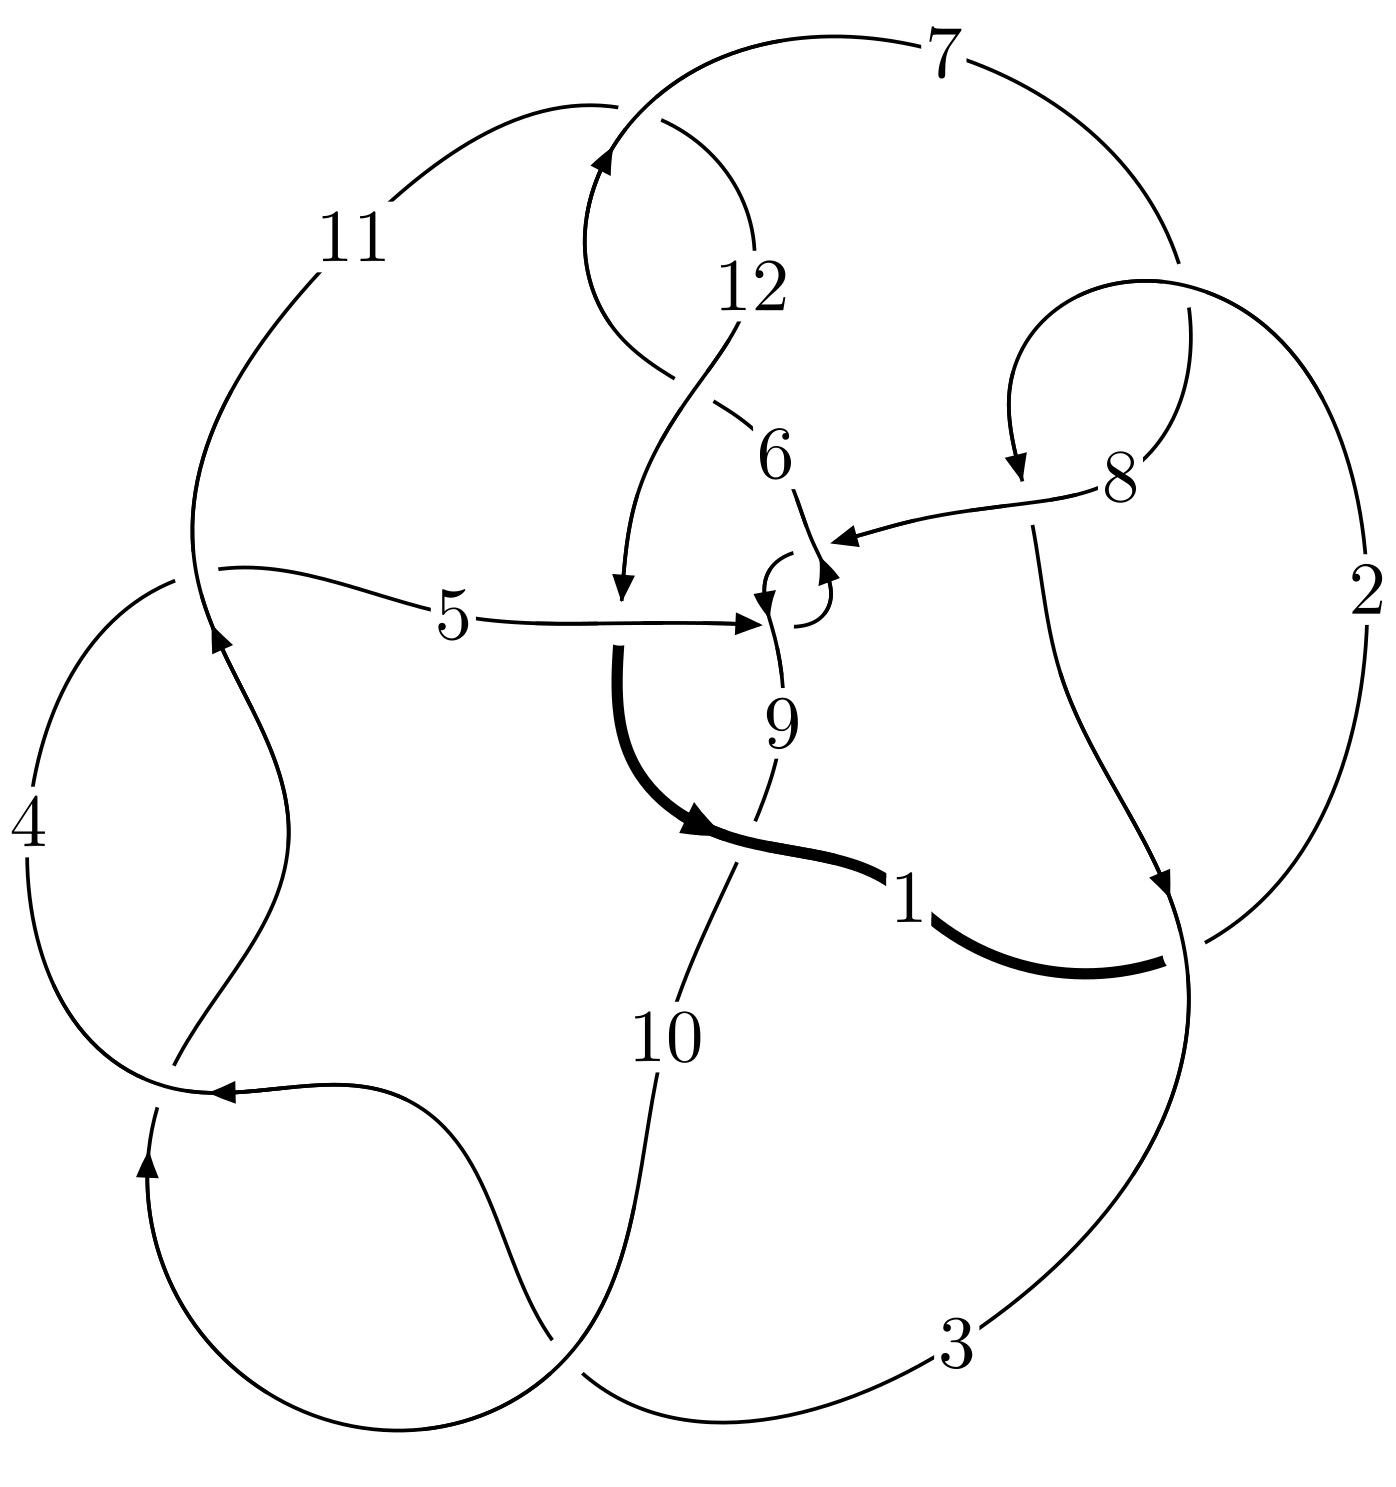
\includegraphics[width=112pt]{../../../GIT/diagram.site/Diagrams/png/1557_12a_0756.png}\\
\ \ \ A knot diagram\footnotemark}&
\allowdisplaybreaks
\textbf{Linearized knot diagam} \\
\cline{2-2}
 &
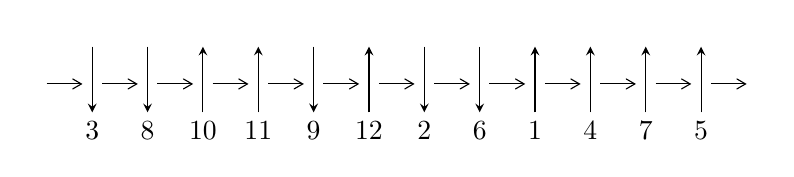
\begin{tikzpicture}[x=20pt, y=17pt]
	% nodes
	\node (C0) at (0, 0) {};
	\node (C1) at (1, 0) {};
	\node (C1U) at (1, +1) {};
	\node (C1D) at (1, -1) {3};

	\node (C2) at (2, 0) {};
	\node (C2U) at (2, +1) {};
	\node (C2D) at (2, -1) {8};

	\node (C3) at (3, 0) {};
	\node (C3U) at (3, +1) {};
	\node (C3D) at (3, -1) {10};

	\node (C4) at (4, 0) {};
	\node (C4U) at (4, +1) {};
	\node (C4D) at (4, -1) {11};

	\node (C5) at (5, 0) {};
	\node (C5U) at (5, +1) {};
	\node (C5D) at (5, -1) {9};

	\node (C6) at (6, 0) {};
	\node (C6U) at (6, +1) {};
	\node (C6D) at (6, -1) {12};

	\node (C7) at (7, 0) {};
	\node (C7U) at (7, +1) {};
	\node (C7D) at (7, -1) {2};

	\node (C8) at (8, 0) {};
	\node (C8U) at (8, +1) {};
	\node (C8D) at (8, -1) {6};

	\node (C9) at (9, 0) {};
	\node (C9U) at (9, +1) {};
	\node (C9D) at (9, -1) {1};

	\node (C10) at (10, 0) {};
	\node (C10U) at (10, +1) {};
	\node (C10D) at (10, -1) {4};

	\node (C11) at (11, 0) {};
	\node (C11U) at (11, +1) {};
	\node (C11D) at (11, -1) {7};

	\node (C12) at (12, 0) {};
	\node (C12U) at (12, +1) {};
	\node (C12D) at (12, -1) {5};
	\node (C13) at (13, 0) {};

	% arrows
	\draw[->,>={angle 60}]
	(C0) edge (C1) (C1) edge (C2) (C2) edge (C3) (C3) edge (C4) (C4) edge (C5) (C5) edge (C6) (C6) edge (C7) (C7) edge (C8) (C8) edge (C9) (C9) edge (C10) (C10) edge (C11) (C11) edge (C12) (C12) edge (C13) ;	\draw[->,>=stealth]
	(C1U) edge (C1D) (C2U) edge (C2D) (C3D) edge (C3U) (C4D) edge (C4U) (C5U) edge (C5D) (C6D) edge (C6U) (C7U) edge (C7D) (C8U) edge (C8D) (C9D) edge (C9U) (C10D) edge (C10U) (C11D) edge (C11U) (C12D) edge (C12U) ;
	\end{tikzpicture} \\
\hhline{~~} \\& 
\textbf{Solving Sequence} \\ \cline{2-2} 
 &
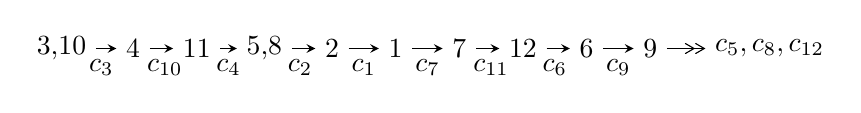
\begin{tikzpicture}[x=23pt, y=7pt]
	% node
	\node (A0) at (-1/8, 0) {3,10};
	\node (A1) at (1, 0) {4};
	\node (A2) at (2, 0) {11};
	\node (A3) at (49/16, 0) {5,8};
	\node (A4) at (33/8, 0) {2};
	\node (A5) at (41/8, 0) {1};
	\node (A6) at (49/8, 0) {7};
	\node (A7) at (57/8, 0) {12};
	\node (A8) at (65/8, 0) {6};
	\node (A9) at (73/8, 0) {9};
	\node (C1) at (1/2, -1) {$c_{3}$};
	\node (C2) at (3/2, -1) {$c_{10}$};
	\node (C3) at (5/2, -1) {$c_{4}$};
	\node (C4) at (29/8, -1) {$c_{2}$};
	\node (C5) at (37/8, -1) {$c_{1}$};
	\node (C6) at (45/8, -1) {$c_{7}$};
	\node (C7) at (53/8, -1) {$c_{11}$};
	\node (C8) at (61/8, -1) {$c_{6}$};
	\node (C9) at (69/8, -1) {$c_{9}$};
	\node (A10) at (11, 0) {$c_{5},c_{8},c_{12}$};

	% edge
	\draw[->,>=stealth]	
	(A0) edge (A1) (A1) edge (A2) (A2) edge (A3) (A3) edge (A4) (A4) edge (A5) (A5) edge (A6) (A6) edge (A7) (A7) edge (A8) (A8) edge (A9) ;
	\draw[->>,>={angle 60}]	
	(A9) edge (A10);
\end{tikzpicture} \\ 

\end{tabular} \\

\footnotetext{
The image of knot diagram is generated by the software ``\textbf{Draw programme}" developed by Andrew Bartholomew(\url{http://www.layer8.co.uk/maths/draw/index.htm\#Running-draw}), where we modified some parts for our purpose(\url{https://github.com/CATsTAILs/LinksPainter}).
}\phantom \\ \newline 
\centering \textbf{Ideals for irreducible components\footnotemark of $X_{\text{par}}$} 
 
\begin{align*}
I^u_{1}&=\langle 
-1.63385\times10^{330} u^{124}-1.41764\times10^{330} u^{123}+\cdots+1.29035\times10^{328} b+9.70787\times10^{330},\\
\phantom{I^u_{1}}&\phantom{= \langle  }6.48012\times10^{331} u^{124}+5.24624\times10^{331} u^{123}+\cdots+1.29035\times10^{328} a-3.36479\times10^{332},\;u^{125}+u^{124}+\cdots-39 u-1\rangle \\
I^u_{2}&=\langle 
469 u^{31}-142 u^{30}+\cdots+293 b+474,\;-1355 u^{31}+717 u^{30}+\cdots+293 a-2414,\\
\phantom{I^u_{2}}&\phantom{= \langle  }u^{32}-18 u^{30}+\cdots-4 u^2+1\rangle \\
\\
\end{align*}
\raggedright * 2 irreducible components of $\dim_{\mathbb{C}}=0$, with total 157 representations.\\
\footnotetext{All coefficients of polynomials are rational numbers. But the coefficients are sometimes approximated in decimal forms when there is not enough margin.}
\newpage
\renewcommand{\arraystretch}{1}
\centering \section*{I. $I^u_{1}= \langle -1.63\times10^{330} u^{124}-1.42\times10^{330} u^{123}+\cdots+1.29\times10^{328} b+9.71\times10^{330},\;6.48\times10^{331} u^{124}+5.25\times10^{331} u^{123}+\cdots+1.29\times10^{328} a-3.36\times10^{332},\;u^{125}+u^{124}+\cdots-39 u-1 \rangle$}
\flushleft \textbf{(i) Arc colorings}\\
\begin{tabular}{m{7pt} m{180pt} m{7pt} m{180pt} }
\flushright $a_{3}=$&$\begin{pmatrix}1\\0\end{pmatrix}$ \\
\flushright $a_{10}=$&$\begin{pmatrix}0\\u\end{pmatrix}$ \\
\flushright $a_{4}=$&$\begin{pmatrix}1\\- u^2\end{pmatrix}$ \\
\flushright $a_{11}=$&$\begin{pmatrix}u\\- u^3+u\end{pmatrix}$ \\
\flushright $a_{5}=$&$\begin{pmatrix}- u^2+1\\u^4-2 u^2\end{pmatrix}$ \\
\flushright $a_{8}=$&$\begin{pmatrix}-5021.98 u^{124}-4065.74 u^{123}+\cdots+883332. u+26076.5\\126.621 u^{124}+109.865 u^{123}+\cdots-25537.3 u-752.343\end{pmatrix}$ \\
\flushright $a_{2}=$&$\begin{pmatrix}-4001.75 u^{124}-3223.53 u^{123}+\cdots+698858. u+20642.5\\-37.9296 u^{124}-8.33395 u^{123}+\cdots-10819.9 u-389.924\end{pmatrix}$ \\
\flushright $a_{1}=$&$\begin{pmatrix}-4039.68 u^{124}-3231.87 u^{123}+\cdots+688038. u+20252.5\\-37.9296 u^{124}-8.33395 u^{123}+\cdots-10819.9 u-389.924\end{pmatrix}$ \\
\flushright $a_{7}=$&$\begin{pmatrix}-1453.38 u^{124}-1154.59 u^{123}+\cdots+246407. u+7265.27\\471.963 u^{124}+369.067 u^{123}+\cdots-66258.7 u-1840.77\end{pmatrix}$ \\
\flushright $a_{12}=$&$\begin{pmatrix}-3723.02 u^{124}-2997.80 u^{123}+\cdots+649734. u+19189.7\\-82.0694 u^{124}-41.9836 u^{123}+\cdots-4543.04 u-212.025\end{pmatrix}$ \\
\flushright $a_{6}=$&$\begin{pmatrix}-5194.57 u^{124}-4244.77 u^{123}+\cdots+953249. u+28426.4\\-69.1566 u^{124}-74.0379 u^{123}+\cdots+28810.1 u+944.086\end{pmatrix}$ \\
\flushright $a_{9}=$&$\begin{pmatrix}3626.15 u^{124}+3080.15 u^{123}+\cdots-754222. u-22905.4\\523.574 u^{124}+441.914 u^{123}+\cdots-104441. u-3131.93\end{pmatrix}$\\&\end{tabular}
\flushleft \textbf{(ii) Obstruction class $= -1$}\\~\\
\flushleft \textbf{(iii) Cusp Shapes $= -10077.2 u^{124}-8235.08 u^{123}+\cdots+1.77727\times10^{6} u+52146.8$}\\~\\
\newpage\renewcommand{\arraystretch}{1}
\flushleft \textbf{(iv) u-Polynomials at the component}\newline \\
\begin{tabular}{m{50pt}|m{274pt}}
Crossings & \hspace{64pt}u-Polynomials at each crossing \\
\hline $$\begin{aligned}c_{1}\end{aligned}$$&$\begin{aligned}
&u^{125}+49 u^{124}+\cdots+9905408 u+295936
\end{aligned}$\\
\hline $$\begin{aligned}c_{2},c_{7}\end{aligned}$$&$\begin{aligned}
&u^{125}+u^{124}+\cdots-1072 u-544
\end{aligned}$\\
\hline $$\begin{aligned}c_{3},c_{4},c_{10}\end{aligned}$$&$\begin{aligned}
&u^{125}+u^{124}+\cdots-39 u-1
\end{aligned}$\\
\hline $$\begin{aligned}c_{5},c_{8}\end{aligned}$$&$\begin{aligned}
&u^{125}-2 u^{124}+\cdots-10915 u+1369
\end{aligned}$\\
\hline $$\begin{aligned}c_{6},c_{11}\end{aligned}$$&$\begin{aligned}
&u^{125}+u^{124}+\cdots-614 u-129
\end{aligned}$\\
\hline $$\begin{aligned}c_{9}\end{aligned}$$&$\begin{aligned}
&u^{125}-7 u^{124}+\cdots-597974523 u+137487799
\end{aligned}$\\
\hline $$\begin{aligned}c_{12}\end{aligned}$$&$\begin{aligned}
&u^{125}-5 u^{124}+\cdots+2718423 u-646429
\end{aligned}$\\
\hline
\end{tabular}\\~\\
\newpage\renewcommand{\arraystretch}{1}
\flushleft \textbf{(v) Riley Polynomials at the component}\newline \\
\begin{tabular}{m{50pt}|m{274pt}}
Crossings & \hspace{64pt}Riley Polynomials at each crossing \\
\hline $$\begin{aligned}c_{1}\end{aligned}$$&$\begin{aligned}
&y^{125}+71 y^{124}+\cdots-2183472283648 y-87578116096
\end{aligned}$\\
\hline $$\begin{aligned}c_{2},c_{7}\end{aligned}$$&$\begin{aligned}
&y^{125}-49 y^{124}+\cdots+9905408 y-295936
\end{aligned}$\\
\hline $$\begin{aligned}c_{3},c_{4},c_{10}\end{aligned}$$&$\begin{aligned}
&y^{125}-129 y^{124}+\cdots+123 y-1
\end{aligned}$\\
\hline $$\begin{aligned}c_{5},c_{8}\end{aligned}$$&$\begin{aligned}
&y^{125}+76 y^{124}+\cdots-60105945 y-1874161
\end{aligned}$\\
\hline $$\begin{aligned}c_{6},c_{11}\end{aligned}$$&$\begin{aligned}
&y^{125}+67 y^{124}+\cdots-1021106 y-16641
\end{aligned}$\\
\hline $$\begin{aligned}c_{9}\end{aligned}$$&$\begin{aligned}
&y^{125}-53 y^{124}+\cdots+628976017143595697 y-18902894873864401
\end{aligned}$\\
\hline $$\begin{aligned}c_{12}\end{aligned}$$&$\begin{aligned}
&y^{125}-25 y^{124}+\cdots+4561628210455 y-417870452041
\end{aligned}$\\
\hline
\end{tabular}\\~\\
\newpage\flushleft \textbf{(vi) Complex Volumes and Cusp Shapes}
$$\begin{array}{c|c|c}  
\text{Solutions to }I^u_{1}& \I (\text{vol} + \sqrt{-1}CS) & \text{Cusp shape}\\
 \hline 
\begin{aligned}
u &= -0.560070 + 0.830618 I \\
a &= \phantom{-}0.005726 + 0.557264 I \\
b &= \phantom{-}0.638215 - 0.682382 I\end{aligned}
 & -0.99708 - 2.04417 I & \phantom{-0.000000 } 0 \\ \hline\begin{aligned}
u &= -0.560070 - 0.830618 I \\
a &= \phantom{-}0.005726 - 0.557264 I \\
b &= \phantom{-}0.638215 + 0.682382 I\end{aligned}
 & -0.99708 + 2.04417 I & \phantom{-0.000000 } 0 \\ \hline\begin{aligned}
u &= -0.522093 + 0.835666 I \\
a &= \phantom{-}0.868028 - 1.000420 I \\
b &= \phantom{-}0.675904 + 0.675750 I\end{aligned}
 & \phantom{-}2.86252 + 2.82941 I & \phantom{-0.000000 } 0 \\ \hline\begin{aligned}
u &= -0.522093 - 0.835666 I \\
a &= \phantom{-}0.868028 + 1.000420 I \\
b &= \phantom{-}0.675904 - 0.675750 I\end{aligned}
 & \phantom{-}2.86252 - 2.82941 I & \phantom{-0.000000 } 0 \\ \hline\begin{aligned}
u &= -0.766804 + 0.684858 I \\
a &= -0.75095 + 1.45806 I \\
b &= -0.793488 - 0.543772 I\end{aligned}
 & -0.41768 - 3.51081 I & \phantom{-0.000000 } 0 \\ \hline\begin{aligned}
u &= -0.766804 - 0.684858 I \\
a &= -0.75095 - 1.45806 I \\
b &= -0.793488 + 0.543772 I\end{aligned}
 & -0.41768 + 3.51081 I & \phantom{-0.000000 } 0 \\ \hline\begin{aligned}
u &= \phantom{-}0.952983 + 0.413336 I \\
a &= \phantom{-}0.56168 - 1.41133 I \\
b &= -1.023360 + 0.155541 I\end{aligned}
 & -1.25962 - 2.31481 I & \phantom{-0.000000 } 0 \\ \hline\begin{aligned}
u &= \phantom{-}0.952983 - 0.413336 I \\
a &= \phantom{-}0.56168 + 1.41133 I \\
b &= -1.023360 - 0.155541 I\end{aligned}
 & -1.25962 + 2.31481 I & \phantom{-0.000000 } 0 \\ \hline\begin{aligned}
u &= \phantom{-}0.526064 + 0.898950 I \\
a &= -0.683296 - 1.126120 I \\
b &= -1.095740 + 0.689568 I\end{aligned}
 & \phantom{-}1.40579 + 13.87260 I & \phantom{-0.000000 } 0 \\ \hline\begin{aligned}
u &= \phantom{-}0.526064 - 0.898950 I \\
a &= -0.683296 + 1.126120 I \\
b &= -1.095740 - 0.689568 I\end{aligned}
 & \phantom{-}1.40579 - 13.87260 I & \phantom{-0.000000 } 0\\
 \hline 
 \end{array}$$\newpage$$\begin{array}{c|c|c}  
\text{Solutions to }I^u_{1}& \I (\text{vol} + \sqrt{-1}CS) & \text{Cusp shape}\\
 \hline 
\begin{aligned}
u &= -0.574092 + 0.756910 I \\
a &= \phantom{-}0.177973 - 0.420259 I \\
b &= -0.528567 + 0.876131 I\end{aligned}
 & \phantom{-}3.11164 - 8.07591 I & \phantom{-0.000000 } 0 \\ \hline\begin{aligned}
u &= -0.574092 - 0.756910 I \\
a &= \phantom{-}0.177973 + 0.420259 I \\
b &= -0.528567 - 0.876131 I\end{aligned}
 & \phantom{-}3.11164 + 8.07591 I & \phantom{-0.000000 } 0 \\ \hline\begin{aligned}
u &= \phantom{-}0.470946 + 0.980198 I \\
a &= \phantom{-}0.557346 + 1.056750 I \\
b &= \phantom{-}1.005970 - 0.651704 I\end{aligned}
 & -2.09362 + 7.24326 I & \phantom{-0.000000 } 0 \\ \hline\begin{aligned}
u &= \phantom{-}0.470946 - 0.980198 I \\
a &= \phantom{-}0.557346 - 1.056750 I \\
b &= \phantom{-}1.005970 + 0.651704 I\end{aligned}
 & -2.09362 - 7.24326 I & \phantom{-0.000000 } 0 \\ \hline\begin{aligned}
u &= \phantom{-}0.716743 + 0.877059 I \\
a &= -0.116982 - 0.199348 I \\
b &= \phantom{-}0.990435 + 0.643096 I\end{aligned}
 & \phantom{-}1.90273 - 7.96364 I & \phantom{-0.000000 } 0 \\ \hline\begin{aligned}
u &= \phantom{-}0.716743 - 0.877059 I \\
a &= -0.116982 + 0.199348 I \\
b &= \phantom{-}0.990435 - 0.643096 I\end{aligned}
 & \phantom{-}1.90273 + 7.96364 I & \phantom{-0.000000 } 0 \\ \hline\begin{aligned}
u &= \phantom{-}0.584208 + 0.610604 I \\
a &= -0.554282 + 0.009632 I \\
b &= \phantom{-}0.686207 + 0.758646 I\end{aligned}
 & \phantom{-}5.48584 + 2.08617 I & \phantom{-0.000000 } 0 \\ \hline\begin{aligned}
u &= \phantom{-}0.584208 - 0.610604 I \\
a &= -0.554282 - 0.009632 I \\
b &= \phantom{-}0.686207 - 0.758646 I\end{aligned}
 & \phantom{-}5.48584 - 2.08617 I & \phantom{-0.000000 } 0 \\ \hline\begin{aligned}
u &= -1.145640 + 0.206937 I \\
a &= -1.157130 + 0.045348 I \\
b &= -0.507097 - 0.326991 I\end{aligned}
 & \phantom{-}3.88412 - 5.25444 I & \phantom{-0.000000 } 0 \\ \hline\begin{aligned}
u &= -1.145640 - 0.206937 I \\
a &= -1.157130 - 0.045348 I \\
b &= -0.507097 + 0.326991 I\end{aligned}
 & \phantom{-}3.88412 + 5.25444 I & \phantom{-0.000000 } 0\\
 \hline 
 \end{array}$$\newpage$$\begin{array}{c|c|c}  
\text{Solutions to }I^u_{1}& \I (\text{vol} + \sqrt{-1}CS) & \text{Cusp shape}\\
 \hline 
\begin{aligned}
u &= -1.165430 + 0.091842 I \\
a &= \phantom{-}0.728158 - 0.555600 I \\
b &= \phantom{-}1.101850 + 0.466236 I\end{aligned}
 & \phantom{-}0.33460 - 5.32985 I & \phantom{-0.000000 } 0 \\ \hline\begin{aligned}
u &= -1.165430 - 0.091842 I \\
a &= \phantom{-}0.728158 + 0.555600 I \\
b &= \phantom{-}1.101850 - 0.466236 I\end{aligned}
 & \phantom{-}0.33460 + 5.32985 I & \phantom{-0.000000 } 0 \\ \hline\begin{aligned}
u &= -0.749603 + 0.352544 I \\
a &= \phantom{-}0.337914 + 1.263390 I \\
b &= \phantom{-}0.471834 - 0.145078 I\end{aligned}
 & -1.55105 - 1.59703 I & \phantom{-0.000000 } 0 \\ \hline\begin{aligned}
u &= -0.749603 - 0.352544 I \\
a &= \phantom{-}0.337914 - 1.263390 I \\
b &= \phantom{-}0.471834 + 0.145078 I\end{aligned}
 & -1.55105 + 1.59703 I & \phantom{-0.000000 } 0 \\ \hline\begin{aligned}
u &= -0.666409 + 0.452542 I \\
a &= -0.94981 + 1.66830 I \\
b &= -0.842878 - 0.409913 I\end{aligned}
 & -0.39342 - 3.59527 I & \phantom{-0.000000 } 0 \\ \hline\begin{aligned}
u &= -0.666409 - 0.452542 I \\
a &= -0.94981 - 1.66830 I \\
b &= -0.842878 + 0.409913 I\end{aligned}
 & -0.39342 + 3.59527 I & \phantom{-0.000000 } 0 \\ \hline\begin{aligned}
u &= -0.445649 + 0.668121 I \\
a &= \phantom{-}1.35812 - 1.35621 I \\
b &= \phantom{-}0.987473 + 0.682486 I\end{aligned}
 & \phantom{-}4.57341 - 7.56022 I & \phantom{-0.000000 } 0 \\ \hline\begin{aligned}
u &= -0.445649 - 0.668121 I \\
a &= \phantom{-}1.35812 + 1.35621 I \\
b &= \phantom{-}0.987473 - 0.682486 I\end{aligned}
 & \phantom{-}4.57341 + 7.56022 I & \phantom{-0.000000 } 0 \\ \hline\begin{aligned}
u &= \phantom{-}0.318208 + 0.730456 I \\
a &= -0.680030 - 0.855887 I \\
b &= -0.849369 + 0.756483 I\end{aligned}
 & \phantom{-}4.68328 + 2.26812 I & \phantom{-0.000000 } 0 \\ \hline\begin{aligned}
u &= \phantom{-}0.318208 - 0.730456 I \\
a &= -0.680030 + 0.855887 I \\
b &= -0.849369 - 0.756483 I\end{aligned}
 & \phantom{-}4.68328 - 2.26812 I & \phantom{-0.000000 } 0\\
 \hline 
 \end{array}$$\newpage$$\begin{array}{c|c|c}  
\text{Solutions to }I^u_{1}& \I (\text{vol} + \sqrt{-1}CS) & \text{Cusp shape}\\
 \hline 
\begin{aligned}
u &= \phantom{-}0.117992 + 0.778543 I \\
a &= -0.745560 + 0.488532 I \\
b &= -1.044850 - 0.052298 I\end{aligned}
 & -5.84195 + 1.29047 I & \phantom{-0.000000 } 0 \\ \hline\begin{aligned}
u &= \phantom{-}0.117992 - 0.778543 I \\
a &= -0.745560 - 0.488532 I \\
b &= -1.044850 + 0.052298 I\end{aligned}
 & -5.84195 - 1.29047 I & \phantom{-0.000000 } 0 \\ \hline\begin{aligned}
u &= \phantom{-}0.929508 + 0.812838 I \\
a &= \phantom{-}0.304121 + 0.383870 I \\
b &= -0.907528 - 0.588471 I\end{aligned}
 & -0.789159 - 1.059320 I & \phantom{-0.000000 } 0 \\ \hline\begin{aligned}
u &= \phantom{-}0.929508 - 0.812838 I \\
a &= \phantom{-}0.304121 - 0.383870 I \\
b &= -0.907528 + 0.588471 I\end{aligned}
 & -0.789159 + 1.059320 I & \phantom{-0.000000 } 0 \\ \hline\begin{aligned}
u &= -0.681221 + 0.250791 I \\
a &= \phantom{-}0.391398 - 0.974536 I \\
b &= \phantom{-}1.145420 + 0.617855 I\end{aligned}
 & -0.01058 - 5.49855 I & \phantom{-0.000000 } 0 \\ \hline\begin{aligned}
u &= -0.681221 - 0.250791 I \\
a &= \phantom{-}0.391398 + 0.974536 I \\
b &= \phantom{-}1.145420 - 0.617855 I\end{aligned}
 & -0.01058 + 5.49855 I & \phantom{-0.000000 } 0 \\ \hline\begin{aligned}
u &= -0.114227 + 0.716514 I \\
a &= -0.985080 + 0.777489 I \\
b &= -0.877419 + 0.522652 I\end{aligned}
 & -2.38804 + 2.09884 I & \phantom{-0.000000 } 0 \\ \hline\begin{aligned}
u &= -0.114227 - 0.716514 I \\
a &= -0.985080 - 0.777489 I \\
b &= -0.877419 - 0.522652 I\end{aligned}
 & -2.38804 - 2.09884 I & \phantom{-0.000000 } 0 \\ \hline\begin{aligned}
u &= -0.366763 + 0.612661 I \\
a &= -0.263955 - 0.210363 I \\
b &= -0.881588 + 0.774174 I\end{aligned}
 & \phantom{-}4.60862 + 3.48554 I & \phantom{-0.000000 } 0 \\ \hline\begin{aligned}
u &= -0.366763 - 0.612661 I \\
a &= -0.263955 + 0.210363 I \\
b &= -0.881588 - 0.774174 I\end{aligned}
 & \phantom{-}4.60862 - 3.48554 I & \phantom{-0.000000 } 0\\
 \hline 
 \end{array}$$\newpage$$\begin{array}{c|c|c}  
\text{Solutions to }I^u_{1}& \I (\text{vol} + \sqrt{-1}CS) & \text{Cusp shape}\\
 \hline 
\begin{aligned}
u &= \phantom{-}0.684821 + 0.192674 I \\
a &= \phantom{-}0.191778 + 0.641827 I \\
b &= \phantom{-}0.189140 - 0.835048 I\end{aligned}
 & \phantom{-}2.75381 - 0.24097 I & \phantom{-0.000000 } 0 \\ \hline\begin{aligned}
u &= \phantom{-}0.684821 - 0.192674 I \\
a &= \phantom{-}0.191778 - 0.641827 I \\
b &= \phantom{-}0.189140 + 0.835048 I\end{aligned}
 & \phantom{-}2.75381 + 0.24097 I & \phantom{-0.000000 } 0 \\ \hline\begin{aligned}
u &= \phantom{-}1.171860 + 0.550693 I \\
a &= -0.113413 + 1.195930 I \\
b &= \phantom{-}0.889439 - 0.246879 I\end{aligned}
 & -2.73540 + 3.43854 I & \phantom{-0.000000 } 0 \\ \hline\begin{aligned}
u &= \phantom{-}1.171860 - 0.550693 I \\
a &= -0.113413 - 1.195930 I \\
b &= \phantom{-}0.889439 + 0.246879 I\end{aligned}
 & -2.73540 - 3.43854 I & \phantom{-0.000000 } 0 \\ \hline\begin{aligned}
u &= -1.300470 + 0.054758 I \\
a &= -0.503238 + 1.222800 I \\
b &= -1.173770 - 0.449089 I\end{aligned}
 & \phantom{-}0.52150 - 2.48167 I & \phantom{-0.000000 } 0 \\ \hline\begin{aligned}
u &= -1.300470 - 0.054758 I \\
a &= -0.503238 - 1.222800 I \\
b &= -1.173770 + 0.449089 I\end{aligned}
 & \phantom{-}0.52150 + 2.48167 I & \phantom{-0.000000 } 0 \\ \hline\begin{aligned}
u &= -0.563295 + 0.410456 I \\
a &= -0.73797 + 1.46376 I \\
b &= -1.130870 - 0.461304 I\end{aligned}
 & -1.01038 - 3.73149 I & \phantom{-0.000000 } 0 \\ \hline\begin{aligned}
u &= -0.563295 - 0.410456 I \\
a &= -0.73797 - 1.46376 I \\
b &= -1.130870 + 0.461304 I\end{aligned}
 & -1.01038 + 3.73149 I & \phantom{-0.000000 } 0 \\ \hline\begin{aligned}
u &= \phantom{-}1.295980 + 0.276425 I \\
a &= -0.104844 + 0.406230 I \\
b &= \phantom{-}0.667351 + 0.431985 I\end{aligned}
 & \phantom{-}1.97854 + 1.51991 I & \phantom{-0.000000 } 0 \\ \hline\begin{aligned}
u &= \phantom{-}1.295980 - 0.276425 I \\
a &= -0.104844 - 0.406230 I \\
b &= \phantom{-}0.667351 - 0.431985 I\end{aligned}
 & \phantom{-}1.97854 - 1.51991 I & \phantom{-0.000000 } 0\\
 \hline 
 \end{array}$$\newpage$$\begin{array}{c|c|c}  
\text{Solutions to }I^u_{1}& \I (\text{vol} + \sqrt{-1}CS) & \text{Cusp shape}\\
 \hline 
\begin{aligned}
u &= \phantom{-}1.321440 + 0.252713 I \\
a &= \phantom{-}0.229971 - 0.530094 I \\
b &= -0.991752 - 0.302605 I\end{aligned}
 & \phantom{-}2.20410 + 2.63018 I & \phantom{-0.000000 } 0 \\ \hline\begin{aligned}
u &= \phantom{-}1.321440 - 0.252713 I \\
a &= \phantom{-}0.229971 + 0.530094 I \\
b &= -0.991752 + 0.302605 I\end{aligned}
 & \phantom{-}2.20410 - 2.63018 I & \phantom{-0.000000 } 0 \\ \hline\begin{aligned}
u &= -1.334000 + 0.230857 I \\
a &= -0.010917 - 0.275692 I \\
b &= \phantom{-}1.206230 + 0.109276 I\end{aligned}
 & -1.31497 - 4.81685 I & \phantom{-0.000000 } 0 \\ \hline\begin{aligned}
u &= -1.334000 - 0.230857 I \\
a &= -0.010917 + 0.275692 I \\
b &= \phantom{-}1.206230 - 0.109276 I\end{aligned}
 & -1.31497 + 4.81685 I & \phantom{-0.000000 } 0 \\ \hline\begin{aligned}
u &= \phantom{-}0.207239 + 0.608895 I \\
a &= \phantom{-}0.887015 - 0.326481 I \\
b &= \phantom{-}1.270940 - 0.040167 I\end{aligned}
 & -3.49592 + 5.99439 I & \phantom{-0.000000 } 0 \\ \hline\begin{aligned}
u &= \phantom{-}0.207239 - 0.608895 I \\
a &= \phantom{-}0.887015 + 0.326481 I \\
b &= \phantom{-}1.270940 + 0.040167 I\end{aligned}
 & -3.49592 - 5.99439 I & \phantom{-0.000000 } 0 \\ \hline\begin{aligned}
u &= -0.160001 + 0.619308 I \\
a &= \phantom{-}1.139030 - 0.725126 I \\
b &= \phantom{-}1.062110 - 0.364198 I\end{aligned}
 & -2.40336 + 0.58212 I & \phantom{-0.000000 } 0 \\ \hline\begin{aligned}
u &= -0.160001 - 0.619308 I \\
a &= \phantom{-}1.139030 + 0.725126 I \\
b &= \phantom{-}1.062110 + 0.364198 I\end{aligned}
 & -2.40336 - 0.58212 I & \phantom{-0.000000 } 0 \\ \hline\begin{aligned}
u &= \phantom{-}1.36461\phantom{ +0.000000I} \\
a &= -0.201345\phantom{ +0.000000I} \\
b &= -1.09759\phantom{ +0.000000I}\end{aligned}
 & \phantom{-}2.85484\phantom{ +0.000000I} & \phantom{-0.000000 } 0 \\ \hline\begin{aligned}
u &= -1.386170 + 0.008339 I \\
a &= \phantom{-}0.44783 + 2.17065 I \\
b &= -0.913799 - 0.669271 I\end{aligned}
 & \phantom{-}2.83268 - 1.28287 I & \phantom{-0.000000 } 0\\
 \hline 
 \end{array}$$\newpage$$\begin{array}{c|c|c}  
\text{Solutions to }I^u_{1}& \I (\text{vol} + \sqrt{-1}CS) & \text{Cusp shape}\\
 \hline 
\begin{aligned}
u &= -1.386170 - 0.008339 I \\
a &= \phantom{-}0.44783 - 2.17065 I \\
b &= -0.913799 + 0.669271 I\end{aligned}
 & \phantom{-}2.83268 + 1.28287 I & \phantom{-0.000000 } 0 \\ \hline\begin{aligned}
u &= -1.388640 + 0.024356 I \\
a &= -1.04296 + 2.29329 I \\
b &= \phantom{-}0.722162 - 0.581090 I\end{aligned}
 & \phantom{-}4.76840 - 3.49617 I & \phantom{-0.000000 } 0 \\ \hline\begin{aligned}
u &= -1.388640 - 0.024356 I \\
a &= -1.04296 - 2.29329 I \\
b &= \phantom{-}0.722162 + 0.581090 I\end{aligned}
 & \phantom{-}4.76840 + 3.49617 I & \phantom{-0.000000 } 0 \\ \hline\begin{aligned}
u &= \phantom{-}1.390110 + 0.044785 I \\
a &= \phantom{-}0.409417 - 0.865522 I \\
b &= -0.202973 + 0.810809 I\end{aligned}
 & \phantom{-}3.62840 + 2.12031 I & \phantom{-0.000000 } 0 \\ \hline\begin{aligned}
u &= \phantom{-}1.390110 - 0.044785 I \\
a &= \phantom{-}0.409417 + 0.865522 I \\
b &= -0.202973 - 0.810809 I\end{aligned}
 & \phantom{-}3.62840 - 2.12031 I & \phantom{-0.000000 } 0 \\ \hline\begin{aligned}
u &= -1.399420 + 0.045549 I \\
a &= -0.54545 - 1.88034 I \\
b &= \phantom{-}1.11231 + 0.99003 I\end{aligned}
 & \phantom{-}8.51763 - 4.17105 I & \phantom{-0.000000 } 0 \\ \hline\begin{aligned}
u &= -1.399420 - 0.045549 I \\
a &= -0.54545 + 1.88034 I \\
b &= \phantom{-}1.11231 - 0.99003 I\end{aligned}
 & \phantom{-}8.51763 + 4.17105 I & \phantom{-0.000000 } 0 \\ \hline\begin{aligned}
u &= \phantom{-}0.574493 + 0.157884 I \\
a &= \phantom{-}0.606746 + 0.361121 I \\
b &= -0.421532 - 0.396092 I\end{aligned}
 & \phantom{-}1.011430 + 0.226694 I & \phantom{-0.000000 } 0 \\ \hline\begin{aligned}
u &= \phantom{-}0.574493 - 0.157884 I \\
a &= \phantom{-}0.606746 - 0.361121 I \\
b &= -0.421532 + 0.396092 I\end{aligned}
 & \phantom{-}1.011430 - 0.226694 I & \phantom{-0.000000 } 0 \\ \hline\begin{aligned}
u &= -1.41252 + 0.17057 I \\
a &= \phantom{-}0.437694 + 0.475558 I \\
b &= -1.49767 - 0.14692 I\end{aligned}
 & \phantom{-}1.71323 - 8.66640 I & \phantom{-0.000000 } 0\\
 \hline 
 \end{array}$$\newpage$$\begin{array}{c|c|c}  
\text{Solutions to }I^u_{1}& \I (\text{vol} + \sqrt{-1}CS) & \text{Cusp shape}\\
 \hline 
\begin{aligned}
u &= -1.41252 - 0.17057 I \\
a &= \phantom{-}0.437694 - 0.475558 I \\
b &= -1.49767 + 0.14692 I\end{aligned}
 & \phantom{-}1.71323 + 8.66640 I & \phantom{-0.000000 } 0 \\ \hline\begin{aligned}
u &= \phantom{-}1.42990 + 0.04798 I \\
a &= \phantom{-}0.517785 + 0.550231 I \\
b &= \phantom{-}1.107380 - 0.031310 I\end{aligned}
 & \phantom{-}5.93415 + 3.76410 I & \phantom{-0.000000 } 0 \\ \hline\begin{aligned}
u &= \phantom{-}1.42990 - 0.04798 I \\
a &= \phantom{-}0.517785 - 0.550231 I \\
b &= \phantom{-}1.107380 + 0.031310 I\end{aligned}
 & \phantom{-}5.93415 - 3.76410 I & \phantom{-0.000000 } 0 \\ \hline\begin{aligned}
u &= \phantom{-}1.45024 + 0.09542 I \\
a &= \phantom{-}1.17413 - 1.64301 I \\
b &= -0.793055 + 0.649275 I\end{aligned}
 & \phantom{-}3.21590 + 3.84758 I & \phantom{-0.000000 } 0 \\ \hline\begin{aligned}
u &= \phantom{-}1.45024 - 0.09542 I \\
a &= \phantom{-}1.17413 + 1.64301 I \\
b &= -0.793055 - 0.649275 I\end{aligned}
 & \phantom{-}3.21590 - 3.84758 I & \phantom{-0.000000 } 0 \\ \hline\begin{aligned}
u &= \phantom{-}1.45433 + 0.12436 I \\
a &= -0.90741 + 2.22612 I \\
b &= \phantom{-}0.971525 - 0.584749 I\end{aligned}
 & \phantom{-}3.95800 + 8.15493 I & \phantom{-0.000000 } 0 \\ \hline\begin{aligned}
u &= \phantom{-}1.45433 - 0.12436 I \\
a &= -0.90741 - 2.22612 I \\
b &= \phantom{-}0.971525 + 0.584749 I\end{aligned}
 & \phantom{-}3.95800 - 8.15493 I & \phantom{-0.000000 } 0 \\ \hline\begin{aligned}
u &= \phantom{-}1.46094 + 0.02460 I \\
a &= -0.62291 + 1.58596 I \\
b &= \phantom{-}0.67639 - 1.27596 I\end{aligned}
 & \phantom{-}9.83186 + 3.67940 I & \phantom{-0.000000 } 0 \\ \hline\begin{aligned}
u &= \phantom{-}1.46094 - 0.02460 I \\
a &= -0.62291 - 1.58596 I \\
b &= \phantom{-}0.67639 + 1.27596 I\end{aligned}
 & \phantom{-}9.83186 - 3.67940 I & \phantom{-0.000000 } 0 \\ \hline\begin{aligned}
u &= -1.46482 + 0.34435 I \\
a &= \phantom{-}0.01966 - 1.80520 I \\
b &= \phantom{-}0.935755 + 0.825465 I\end{aligned}
 & \phantom{-}10.29070 - 6.34764 I & \phantom{-0.000000 } 0\\
 \hline 
 \end{array}$$\newpage$$\begin{array}{c|c|c}  
\text{Solutions to }I^u_{1}& \I (\text{vol} + \sqrt{-1}CS) & \text{Cusp shape}\\
 \hline 
\begin{aligned}
u &= -1.46482 - 0.34435 I \\
a &= \phantom{-}0.01966 + 1.80520 I \\
b &= \phantom{-}0.935755 - 0.825465 I\end{aligned}
 & \phantom{-}10.29070 + 6.34764 I & \phantom{-0.000000 } 0 \\ \hline\begin{aligned}
u &= \phantom{-}1.49090 + 0.24676 I \\
a &= -0.25178 - 1.91311 I \\
b &= -1.092470 + 0.701219 I\end{aligned}
 & \phantom{-}10.8627 + 10.9335 I & \phantom{-0.000000 } 0 \\ \hline\begin{aligned}
u &= \phantom{-}1.49090 - 0.24676 I \\
a &= -0.25178 + 1.91311 I \\
b &= -1.092470 - 0.701219 I\end{aligned}
 & \phantom{-}10.8627 - 10.9335 I & \phantom{-0.000000 } 0 \\ \hline\begin{aligned}
u &= \phantom{-}1.48613 + 0.28135 I \\
a &= -0.826003 - 1.017160 I \\
b &= \phantom{-}0.863483 + 0.870070 I\end{aligned}
 & \phantom{-}10.53280 + 0.06582 I & \phantom{-0.000000 } 0 \\ \hline\begin{aligned}
u &= \phantom{-}1.48613 - 0.28135 I \\
a &= -0.826003 + 1.017160 I \\
b &= \phantom{-}0.863483 - 0.870070 I\end{aligned}
 & \phantom{-}10.53280 - 0.06582 I & \phantom{-0.000000 } 0 \\ \hline\begin{aligned}
u &= \phantom{-}0.031279 + 0.484384 I \\
a &= \phantom{-}1.29261 - 0.70808 I \\
b &= -0.059153 - 0.541656 I\end{aligned}
 & \phantom{-}0.65818 + 2.61281 I & \phantom{-0.000000 } 0 \\ \hline\begin{aligned}
u &= \phantom{-}0.031279 - 0.484384 I \\
a &= \phantom{-}1.29261 + 0.70808 I \\
b &= -0.059153 + 0.541656 I\end{aligned}
 & \phantom{-}0.65818 - 2.61281 I & \phantom{-0.000000 } 0 \\ \hline\begin{aligned}
u &= -1.53360 + 0.19563 I \\
a &= \phantom{-}0.901457 - 0.881586 I \\
b &= -0.577297 + 0.890051 I\end{aligned}
 & \phantom{-}12.45140 - 5.03884 I & \phantom{-0.000000 } 0 \\ \hline\begin{aligned}
u &= -1.53360 - 0.19563 I \\
a &= \phantom{-}0.901457 + 0.881586 I \\
b &= -0.577297 - 0.890051 I\end{aligned}
 & \phantom{-}12.45140 + 5.03884 I & \phantom{-0.000000 } 0 \\ \hline\begin{aligned}
u &= \phantom{-}1.54095 + 0.12837 I \\
a &= -0.35724 + 1.54219 I \\
b &= \phantom{-}1.215550 - 0.602561 I\end{aligned}
 & \phantom{-}6.00078 + 5.72659 I & \phantom{-0.000000 } 0\\
 \hline 
 \end{array}$$\newpage$$\begin{array}{c|c|c}  
\text{Solutions to }I^u_{1}& \I (\text{vol} + \sqrt{-1}CS) & \text{Cusp shape}\\
 \hline 
\begin{aligned}
u &= \phantom{-}1.54095 - 0.12837 I \\
a &= -0.35724 - 1.54219 I \\
b &= \phantom{-}1.215550 + 0.602561 I\end{aligned}
 & \phantom{-}6.00078 - 5.72659 I & \phantom{-0.000000 } 0 \\ \hline\begin{aligned}
u &= \phantom{-}1.54379 + 0.09192 I \\
a &= \phantom{-}0.60093 - 1.49709 I \\
b &= -1.28320 + 0.84650 I\end{aligned}
 & \phantom{-}7.28577 + 6.85904 I & \phantom{-0.000000 } 0 \\ \hline\begin{aligned}
u &= \phantom{-}1.54379 - 0.09192 I \\
a &= \phantom{-}0.60093 + 1.49709 I \\
b &= -1.28320 - 0.84650 I\end{aligned}
 & \phantom{-}7.28577 - 6.85904 I & \phantom{-0.000000 } 0 \\ \hline\begin{aligned}
u &= -0.284654 + 0.350194 I \\
a &= -0.56372 + 3.72614 I \\
b &= -1.073340 - 0.462416 I\end{aligned}
 & -1.82555 - 6.40335 I & \phantom{-0.000000 -}0. + 12.56791 I \\ \hline\begin{aligned}
u &= -0.284654 - 0.350194 I \\
a &= -0.56372 - 3.72614 I \\
b &= -1.073340 + 0.462416 I\end{aligned}
 & -1.82555 + 6.40335 I & \phantom{-0.000000 } 0. - 12.56791 I \\ \hline\begin{aligned}
u &= \phantom{-}1.53448 + 0.21454 I \\
a &= \phantom{-}0.03631 + 1.77056 I \\
b &= \phantom{-}1.040570 - 0.636265 I\end{aligned}
 & \phantom{-}6.77922 + 6.58251 I & \phantom{-0.000000 } 0 \\ \hline\begin{aligned}
u &= \phantom{-}1.53448 - 0.21454 I \\
a &= \phantom{-}0.03631 - 1.77056 I \\
b &= \phantom{-}1.040570 + 0.636265 I\end{aligned}
 & \phantom{-}6.77922 - 6.58251 I & \phantom{-0.000000 } 0 \\ \hline\begin{aligned}
u &= -1.55767 + 0.01776 I \\
a &= \phantom{-}0.15615 + 1.48985 I \\
b &= -0.259787 - 1.171730 I\end{aligned}
 & \phantom{-}10.25640 - 0.32613 I & \phantom{-0.000000 } 0 \\ \hline\begin{aligned}
u &= -1.55767 - 0.01776 I \\
a &= \phantom{-}0.15615 - 1.48985 I \\
b &= -0.259787 + 1.171730 I\end{aligned}
 & \phantom{-}10.25640 + 0.32613 I & \phantom{-0.000000 } 0 \\ \hline\begin{aligned}
u &= -1.55722 + 0.10507 I \\
a &= -0.711336 + 1.014210 I \\
b &= \phantom{-}0.506428 - 0.739167 I\end{aligned}
 & \phantom{-}8.30090 - 1.37345 I & \phantom{-0.000000 } 0\\
 \hline 
 \end{array}$$\newpage$$\begin{array}{c|c|c}  
\text{Solutions to }I^u_{1}& \I (\text{vol} + \sqrt{-1}CS) & \text{Cusp shape}\\
 \hline 
\begin{aligned}
u &= -1.55722 - 0.10507 I \\
a &= -0.711336 - 1.014210 I \\
b &= \phantom{-}0.506428 + 0.739167 I\end{aligned}
 & \phantom{-}8.30090 + 1.37345 I & \phantom{-0.000000 } 0 \\ \hline\begin{aligned}
u &= \phantom{-}1.53801 + 0.27214 I \\
a &= \phantom{-}0.764294 + 1.117260 I \\
b &= -0.627234 - 0.900488 I\end{aligned}
 & \phantom{-}5.83514 + 5.99338 I & \phantom{-0.000000 } 0 \\ \hline\begin{aligned}
u &= \phantom{-}1.53801 - 0.27214 I \\
a &= \phantom{-}0.764294 - 1.117260 I \\
b &= -0.627234 + 0.900488 I\end{aligned}
 & \phantom{-}5.83514 - 5.99338 I & \phantom{-0.000000 } 0 \\ \hline\begin{aligned}
u &= \phantom{-}1.54556 + 0.25935 I \\
a &= -0.782113 - 1.163170 I \\
b &= \phantom{-}0.558374 + 1.055100 I\end{aligned}
 & \phantom{-}10.0370 + 11.8102 I & \phantom{-0.000000 } 0 \\ \hline\begin{aligned}
u &= \phantom{-}1.54556 - 0.25935 I \\
a &= -0.782113 + 1.163170 I \\
b &= \phantom{-}0.558374 - 1.055100 I\end{aligned}
 & \phantom{-}10.0370 - 11.8102 I & \phantom{-0.000000 } 0 \\ \hline\begin{aligned}
u &= -1.55007 + 0.32187 I \\
a &= -0.03780 - 1.81800 I \\
b &= \phantom{-}1.158870 + 0.755891 I\end{aligned}
 & \phantom{-}8.1406 - 18.3342 I & \phantom{-0.000000 } 0 \\ \hline\begin{aligned}
u &= -1.55007 - 0.32187 I \\
a &= -0.03780 + 1.81800 I \\
b &= \phantom{-}1.158870 - 0.755891 I\end{aligned}
 & \phantom{-}8.1406 + 18.3342 I & \phantom{-0.000000 } 0 \\ \hline\begin{aligned}
u &= -1.54543 + 0.34619 I \\
a &= \phantom{-}0.04293 + 1.78974 I \\
b &= -1.075140 - 0.732250 I\end{aligned}
 & \phantom{-}4.45255 - 12.03210 I & \phantom{-0.000000 } 0 \\ \hline\begin{aligned}
u &= -1.54543 - 0.34619 I \\
a &= \phantom{-}0.04293 - 1.78974 I \\
b &= -1.075140 + 0.732250 I\end{aligned}
 & \phantom{-}4.45255 + 12.03210 I & \phantom{-0.000000 } 0 \\ \hline\begin{aligned}
u &= \phantom{-}1.57451 + 0.28056 I \\
a &= -0.18047 - 1.55731 I \\
b &= -0.912835 + 0.670428 I\end{aligned}
 & \phantom{-}9.79840 + 1.34406 I & \phantom{-0.000000 } 0\\
 \hline 
 \end{array}$$\newpage$$\begin{array}{c|c|c}  
\text{Solutions to }I^u_{1}& \I (\text{vol} + \sqrt{-1}CS) & \text{Cusp shape}\\
 \hline 
\begin{aligned}
u &= \phantom{-}1.57451 - 0.28056 I \\
a &= -0.18047 + 1.55731 I \\
b &= -0.912835 - 0.670428 I\end{aligned}
 & \phantom{-}9.79840 - 1.34406 I & \phantom{-0.000000 } 0 \\ \hline\begin{aligned}
u &= -0.129864 + 0.337557 I \\
a &= \phantom{-}2.18916 - 0.20050 I \\
b &= \phantom{-}0.834121 - 0.293543 I\end{aligned}
 & -1.36503 + 0.96077 I & -2.26477 - 0.76917 I \\ \hline\begin{aligned}
u &= -0.129864 - 0.337557 I \\
a &= \phantom{-}2.18916 + 0.20050 I \\
b &= \phantom{-}0.834121 + 0.293543 I\end{aligned}
 & -1.36503 - 0.96077 I & -2.26477 + 0.76917 I \\ \hline\begin{aligned}
u &= -0.284448 + 0.208008 I \\
a &= -2.38495 - 2.92243 I \\
b &= \phantom{-}0.964406 + 0.463082 I\end{aligned}
 & -2.58416 - 2.59005 I & -0.96655 + 4.26055 I \\ \hline\begin{aligned}
u &= -0.284448 - 0.208008 I \\
a &= -2.38495 + 2.92243 I \\
b &= \phantom{-}0.964406 - 0.463082 I\end{aligned}
 & -2.58416 + 2.59005 I & -0.96655 - 4.26055 I \\ \hline\begin{aligned}
u &= -1.66079 + 0.04111 I \\
a &= -0.765492 + 0.775809 I \\
b &= \phantom{-}0.605364 - 0.404140 I\end{aligned}
 & \phantom{-}8.65952 - 1.61792 I & \phantom{-0.000000 } 0 \\ \hline\begin{aligned}
u &= -1.66079 - 0.04111 I \\
a &= -0.765492 - 0.775809 I \\
b &= \phantom{-}0.605364 + 0.404140 I\end{aligned}
 & \phantom{-}8.65952 + 1.61792 I & \phantom{-0.000000 } 0 \\ \hline\begin{aligned}
u &= -1.67909 + 0.20352 I \\
a &= \phantom{-}0.669467 - 0.807013 I \\
b &= -0.799147 + 0.656332 I\end{aligned}
 & \phantom{-}10.15450 + 3.80654 I & \phantom{-0.000000 } 0 \\ \hline\begin{aligned}
u &= -1.67909 - 0.20352 I \\
a &= \phantom{-}0.669467 + 0.807013 I \\
b &= -0.799147 - 0.656332 I\end{aligned}
 & \phantom{-}10.15450 - 3.80654 I & \phantom{-0.000000 } 0 \\ \hline\begin{aligned}
u &= -0.208967 + 0.119445 I \\
a &= -2.46111 + 2.48479 I \\
b &= \phantom{-}0.544639 + 0.424569 I\end{aligned}
 & -1.46307 - 1.24235 I & -0.09926 + 3.49057 I\\
 \hline 
 \end{array}$$\newpage$$\begin{array}{c|c|c}  
\text{Solutions to }I^u_{1}& \I (\text{vol} + \sqrt{-1}CS) & \text{Cusp shape}\\
 \hline 
\begin{aligned}
u &= -0.208967 - 0.119445 I \\
a &= -2.46111 - 2.48479 I \\
b &= \phantom{-}0.544639 - 0.424569 I\end{aligned}
 & -1.46307 + 1.24235 I & -0.09926 - 3.49057 I \\ \hline\begin{aligned}
u &= -0.185898 + 0.065034 I \\
a &= \phantom{-}0.35462 + 1.40565 I \\
b &= -0.814308 + 1.000220 I\end{aligned}
 & \phantom{-}4.08748 + 3.55759 I & \phantom{-}20.3705 - 11.4990 I \\ \hline\begin{aligned}
u &= -0.185898 - 0.065034 I \\
a &= \phantom{-}0.35462 - 1.40565 I \\
b &= -0.814308 - 1.000220 I\end{aligned}
 & \phantom{-}4.08748 - 3.55759 I & \phantom{-}20.3705 + 11.4990 I \\ \hline\begin{aligned}
u &= -0.180834 + 0.014822 I \\
a &= -6.96058 + 7.53634 I \\
b &= -0.705849 + 0.105967 I\end{aligned}
 & \phantom{-}0.42093 - 3.22495 I & -2.01065 + 9.42270 I \\ \hline\begin{aligned}
u &= -0.180834 - 0.014822 I \\
a &= -6.96058 - 7.53634 I \\
b &= -0.705849 - 0.105967 I\end{aligned}
 & \phantom{-}0.42093 + 3.22495 I & -2.01065 - 9.42270 I\\
 \hline 
 \end{array}$$\newpage\newpage\renewcommand{\arraystretch}{1}
\centering \section*{II. $I^u_{2}= \langle 469 u^{31}-142 u^{30}+\cdots+293 b+474,\;-1355 u^{31}+717 u^{30}+\cdots+293 a-2414,\;u^{32}-18 u^{30}+\cdots-4 u^2+1 \rangle$}
\flushleft \textbf{(i) Arc colorings}\\
\begin{tabular}{m{7pt} m{180pt} m{7pt} m{180pt} }
\flushright $a_{3}=$&$\begin{pmatrix}1\\0\end{pmatrix}$ \\
\flushright $a_{10}=$&$\begin{pmatrix}0\\u\end{pmatrix}$ \\
\flushright $a_{4}=$&$\begin{pmatrix}1\\- u^2\end{pmatrix}$ \\
\flushright $a_{11}=$&$\begin{pmatrix}u\\- u^3+u\end{pmatrix}$ \\
\flushright $a_{5}=$&$\begin{pmatrix}- u^2+1\\u^4-2 u^2\end{pmatrix}$ \\
\flushright $a_{8}=$&$\begin{pmatrix}4.62457 u^{31}-2.44710 u^{30}+\cdots-20.2116 u+8.23891\\-1.60068 u^{31}+0.484642 u^{30}+\cdots+2.06143 u-1.61775\end{pmatrix}$ \\
\flushright $a_{2}=$&$\begin{pmatrix}-6.93857 u^{31}+2.38225 u^{30}+\cdots+26.4710 u-11.4027\\1.13311 u^{31}-0.505119 u^{30}+\cdots-7.97952 u+3.46075\end{pmatrix}$ \\
\flushright $a_{1}=$&$\begin{pmatrix}-5.80546 u^{31}+1.87713 u^{30}+\cdots+18.4915 u-7.94198\\1.13311 u^{31}-0.505119 u^{30}+\cdots-7.97952 u+3.46075\end{pmatrix}$ \\
\flushright $a_{7}=$&$\begin{pmatrix}-3.09215 u^{31}+1.42662 u^{30}+\cdots+15.2935 u-8.39590\\2.80205 u^{31}-2.45392 u^{30}+\cdots-12.1843 u+4.85324\end{pmatrix}$ \\
\flushright $a_{12}=$&$\begin{pmatrix}-5.80546 u^{31}+1.87713 u^{30}+\cdots+17.4915 u-7.94198\\1.13311 u^{31}-0.505119 u^{30}+\cdots-6.97952 u+3.46075\end{pmatrix}$ \\
\flushright $a_{6}=$&$\begin{pmatrix}-2.95563 u^{31}+0.498294 u^{30}+\cdots+14.0068 u-6.84642\\0.416382 u^{31}-2.63140 u^{30}+\cdots+0.525597 u+0.825939\end{pmatrix}$ \\
\flushright $a_{9}=$&$\begin{pmatrix}0.365188 u^{31}-0.283276 u^{30}+\cdots+5.13311 u-0.505119\\2.87713 u^{31}-2.76451 u^{30}+\cdots-8.94198 u+5.80546\end{pmatrix}$\\&\end{tabular}
\flushleft \textbf{(ii) Obstruction class $= 1$}\\~\\
\flushleft \textbf{(iii) Cusp Shapes $= -\frac{2531}{293} u^{31}-\frac{838}{293} u^{30}+\cdots+\frac{12142}{293} u-\frac{5448}{293}$}\\~\\
\newpage\renewcommand{\arraystretch}{1}
\flushleft \textbf{(iv) u-Polynomials at the component}\newline \\
\begin{tabular}{m{50pt}|m{274pt}}
Crossings & \hspace{64pt}u-Polynomials at each crossing \\
\hline $$\begin{aligned}c_{1}\end{aligned}$$&$\begin{aligned}
&u^{32}-16 u^{31}+\cdots-19 u+1
\end{aligned}$\\
\hline $$\begin{aligned}c_{2}\end{aligned}$$&$\begin{aligned}
&u^{32}-8 u^{30}+\cdots+u+1
\end{aligned}$\\
\hline $$\begin{aligned}c_{3},c_{4}\end{aligned}$$&$\begin{aligned}
&u^{32}-18 u^{30}+\cdots-4 u^2+1
\end{aligned}$\\
\hline $$\begin{aligned}c_{5}\end{aligned}$$&$\begin{aligned}
&u^{32}-3 u^{31}+\cdots+10 u^2+1
\end{aligned}$\\
\hline $$\begin{aligned}c_{6}\end{aligned}$$&$\begin{aligned}
&u^{32}+12 u^{30}+\cdots- u+1
\end{aligned}$\\
\hline $$\begin{aligned}c_{7}\end{aligned}$$&$\begin{aligned}
&u^{32}-8 u^{30}+\cdots- u+1
\end{aligned}$\\
\hline $$\begin{aligned}c_{8}\end{aligned}$$&$\begin{aligned}
&u^{32}+3 u^{31}+\cdots+10 u^2+1
\end{aligned}$\\
\hline $$\begin{aligned}c_{9}\end{aligned}$$&$\begin{aligned}
&u^{32}-2 u^{30}+\cdots-3 u^2+1
\end{aligned}$\\
\hline $$\begin{aligned}c_{10}\end{aligned}$$&$\begin{aligned}
&u^{32}-18 u^{30}+\cdots-4 u^2+1
\end{aligned}$\\
\hline $$\begin{aligned}c_{11}\end{aligned}$$&$\begin{aligned}
&u^{32}+12 u^{30}+\cdots+u+1
\end{aligned}$\\
\hline $$\begin{aligned}c_{12}\end{aligned}$$&$\begin{aligned}
&u^{32}-9 u^{29}+\cdots+8 u^2+1
\end{aligned}$\\
\hline
\end{tabular}\\~\\
\newpage\renewcommand{\arraystretch}{1}
\flushleft \textbf{(v) Riley Polynomials at the component}\newline \\
\begin{tabular}{m{50pt}|m{274pt}}
Crossings & \hspace{64pt}Riley Polynomials at each crossing \\
\hline $$\begin{aligned}c_{1}\end{aligned}$$&$\begin{aligned}
&y^{32}+16 y^{31}+\cdots+17 y+1
\end{aligned}$\\
\hline $$\begin{aligned}c_{2},c_{7}\end{aligned}$$&$\begin{aligned}
&y^{32}-16 y^{31}+\cdots-19 y+1
\end{aligned}$\\
\hline $$\begin{aligned}c_{3},c_{4},c_{10}\end{aligned}$$&$\begin{aligned}
&y^{32}-36 y^{31}+\cdots-8 y+1
\end{aligned}$\\
\hline $$\begin{aligned}c_{5},c_{8}\end{aligned}$$&$\begin{aligned}
&y^{32}+17 y^{31}+\cdots+20 y+1
\end{aligned}$\\
\hline $$\begin{aligned}c_{6},c_{11}\end{aligned}$$&$\begin{aligned}
&y^{32}+24 y^{31}+\cdots+29 y+1
\end{aligned}$\\
\hline $$\begin{aligned}c_{9}\end{aligned}$$&$\begin{aligned}
&y^{32}-4 y^{31}+\cdots-6 y+1
\end{aligned}$\\
\hline $$\begin{aligned}c_{12}\end{aligned}$$&$\begin{aligned}
&y^{32}+2 y^{30}+\cdots+16 y+1
\end{aligned}$\\
\hline
\end{tabular}\\~\\
\newpage\flushleft \textbf{(vi) Complex Volumes and Cusp Shapes}
$$\begin{array}{c|c|c}  
\text{Solutions to }I^u_{2}& \I (\text{vol} + \sqrt{-1}CS) & \text{Cusp shape}\\
 \hline 
\begin{aligned}
u &= -0.823229 + 0.573526 I \\
a &= \phantom{-}0.230051 - 1.193660 I \\
b &= \phantom{-}1.001010 + 0.496794 I\end{aligned}
 & -2.09021 - 5.00508 I & \phantom{-}0.32029 + 7.36848 I \\ \hline\begin{aligned}
u &= -0.823229 - 0.573526 I \\
a &= \phantom{-}0.230051 + 1.193660 I \\
b &= \phantom{-}1.001010 - 0.496794 I\end{aligned}
 & -2.09021 + 5.00508 I & \phantom{-}0.32029 - 7.36848 I \\ \hline\begin{aligned}
u &= -0.905331 + 0.410272 I \\
a &= \phantom{-}0.637023 - 0.634846 I \\
b &= -1.030370 + 0.490351 I\end{aligned}
 & -2.15241 + 1.03931 I & -0.740501 - 0.627183 I \\ \hline\begin{aligned}
u &= -0.905331 - 0.410272 I \\
a &= \phantom{-}0.637023 + 0.634846 I \\
b &= -1.030370 - 0.490351 I\end{aligned}
 & -2.15241 - 1.03931 I & -0.740501 + 0.627183 I \\ \hline\begin{aligned}
u &= \phantom{-}0.886661 + 0.571779 I \\
a &= \phantom{-}0.277016 - 0.483095 I \\
b &= \phantom{-}0.686227 + 0.474422 I\end{aligned}
 & -1.00963 + 0.99283 I & \phantom{-}2.87836 + 2.32450 I \\ \hline\begin{aligned}
u &= \phantom{-}0.886661 - 0.571779 I \\
a &= \phantom{-}0.277016 + 0.483095 I \\
b &= \phantom{-}0.686227 - 0.474422 I\end{aligned}
 & -1.00963 - 0.99283 I & \phantom{-}2.87836 - 2.32450 I \\ \hline\begin{aligned}
u &= \phantom{-}0.960413 + 0.497111 I \\
a &= -0.30409 - 1.84527 I \\
b &= -0.655739 + 0.511334 I\end{aligned}
 & -0.86909 + 3.07016 I & -1.325078 - 0.355339 I \\ \hline\begin{aligned}
u &= \phantom{-}0.960413 - 0.497111 I \\
a &= -0.30409 + 1.84527 I \\
b &= -0.655739 - 0.511334 I\end{aligned}
 & -0.86909 - 3.07016 I & -1.325078 + 0.355339 I \\ \hline\begin{aligned}
u &= \phantom{-}1.226110 + 0.132661 I \\
a &= -1.16737 - 1.05240 I \\
b &= -0.739922 - 0.151475 I\end{aligned}
 & \phantom{-}3.21909 + 4.21288 I & \phantom{-}2.38672 - 4.46762 I \\ \hline\begin{aligned}
u &= \phantom{-}1.226110 - 0.132661 I \\
a &= -1.16737 + 1.05240 I \\
b &= -0.739922 + 0.151475 I\end{aligned}
 & \phantom{-}3.21909 - 4.21288 I & \phantom{-}2.38672 + 4.46762 I\\
 \hline 
 \end{array}$$\newpage$$\begin{array}{c|c|c}  
\text{Solutions to }I^u_{2}& \I (\text{vol} + \sqrt{-1}CS) & \text{Cusp shape}\\
 \hline 
\begin{aligned}
u &= -1.250750 + 0.066354 I \\
a &= -0.073988 - 0.215665 I \\
b &= -1.152920 - 0.317190 I\end{aligned}
 & \phantom{-}1.41682 - 6.19666 I & \phantom{-}4.72969 + 6.81735 I \\ \hline\begin{aligned}
u &= -1.250750 - 0.066354 I \\
a &= -0.073988 + 0.215665 I \\
b &= -1.152920 + 0.317190 I\end{aligned}
 & \phantom{-}1.41682 + 6.19666 I & \phantom{-}4.72969 - 6.81735 I \\ \hline\begin{aligned}
u &= -1.284700 + 0.159063 I \\
a &= \phantom{-}0.941075 - 0.385333 I \\
b &= \phantom{-}1.054270 + 0.306052 I\end{aligned}
 & \phantom{-}0.19355 - 3.89178 I & \phantom{-}2.00000 + 2.50362 I \\ \hline\begin{aligned}
u &= -1.284700 - 0.159063 I \\
a &= \phantom{-}0.941075 + 0.385333 I \\
b &= \phantom{-}1.054270 - 0.306052 I\end{aligned}
 & \phantom{-}0.19355 + 3.89178 I & \phantom{-}2.00000 - 2.50362 I \\ \hline\begin{aligned}
u &= \phantom{-}1.331670 + 0.231893 I \\
a &= -0.422062 + 0.851905 I \\
b &= \phantom{-}0.823576 + 0.245895 I\end{aligned}
 & \phantom{-}1.14054 + 1.60622 I & -2.50242 + 0. I\phantom{ +0.000000I} \\ \hline\begin{aligned}
u &= \phantom{-}1.331670 - 0.231893 I \\
a &= -0.422062 - 0.851905 I \\
b &= \phantom{-}0.823576 - 0.245895 I\end{aligned}
 & \phantom{-}1.14054 - 1.60622 I & -2.50242 + 0. I\phantom{ +0.000000I} \\ \hline\begin{aligned}
u &= -0.109844 + 0.592866 I \\
a &= -1.00351 + 1.39190 I \\
b &= -0.921703 + 0.346676 I\end{aligned}
 & -3.36734 + 1.41923 I & -6.06389 - 0.47143 I \\ \hline\begin{aligned}
u &= -0.109844 - 0.592866 I \\
a &= -1.00351 - 1.39190 I \\
b &= -0.921703 - 0.346676 I\end{aligned}
 & -3.36734 - 1.41923 I & -6.06389 + 0.47143 I \\ \hline\begin{aligned}
u &= \phantom{-}0.501084 + 0.247454 I \\
a &= -0.46279 + 3.56984 I \\
b &= \phantom{-}0.647644 - 0.228760 I\end{aligned}
 & \phantom{-}0.68591 - 2.77162 I & \phantom{-}5.96833 - 2.65828 I \\ \hline\begin{aligned}
u &= \phantom{-}0.501084 - 0.247454 I \\
a &= -0.46279 - 3.56984 I \\
b &= \phantom{-}0.647644 + 0.228760 I\end{aligned}
 & \phantom{-}0.68591 + 2.77162 I & \phantom{-}5.96833 + 2.65828 I\\
 \hline 
 \end{array}$$\newpage$$\begin{array}{c|c|c}  
\text{Solutions to }I^u_{2}& \I (\text{vol} + \sqrt{-1}CS) & \text{Cusp shape}\\
 \hline 
\begin{aligned}
u &= \phantom{-}1.44081 + 0.14512 I \\
a &= -0.48645 + 1.82864 I \\
b &= \phantom{-}1.06820 - 0.96421 I\end{aligned}
 & \phantom{-}8.61139 + 5.32683 I & \phantom{-}7.34287 - 6.36655 I \\ \hline\begin{aligned}
u &= \phantom{-}1.44081 - 0.14512 I \\
a &= -0.48645 - 1.82864 I \\
b &= \phantom{-}1.06820 + 0.96421 I\end{aligned}
 & \phantom{-}8.61139 - 5.32683 I & \phantom{-}7.34287 + 6.36655 I \\ \hline\begin{aligned}
u &= -0.464219 + 0.029319 I \\
a &= -1.04008 + 2.30995 I \\
b &= \phantom{-}1.131700 - 0.427011 I\end{aligned}
 & -1.36908 + 5.66549 I & \phantom{-}1.76337 - 5.56166 I \\ \hline\begin{aligned}
u &= -0.464219 - 0.029319 I \\
a &= -1.04008 - 2.30995 I \\
b &= \phantom{-}1.131700 + 0.427011 I\end{aligned}
 & -1.36908 - 5.66549 I & \phantom{-}1.76337 + 5.56166 I \\ \hline\begin{aligned}
u &= -1.54390 + 0.08683 I \\
a &= -0.437146 + 1.308350 I \\
b &= \phantom{-}0.571375 - 1.007390 I\end{aligned}
 & \phantom{-}9.97917 + 1.85409 I & \phantom{-0.000000 } 0 \\ \hline\begin{aligned}
u &= -1.54390 - 0.08683 I \\
a &= -0.437146 - 1.308350 I \\
b &= \phantom{-}0.571375 + 1.007390 I\end{aligned}
 & \phantom{-}9.97917 - 1.85409 I & \phantom{-0.000000 } 0 \\ \hline\begin{aligned}
u &= \phantom{-}1.55180 + 0.09269 I \\
a &= \phantom{-}0.49340 - 1.57704 I \\
b &= -1.185780 + 0.630177 I\end{aligned}
 & \phantom{-}5.90343 + 6.49247 I & \phantom{-0.000000 } 0 \\ \hline\begin{aligned}
u &= \phantom{-}1.55180 - 0.09269 I \\
a &= \phantom{-}0.49340 + 1.57704 I \\
b &= -1.185780 - 0.630177 I\end{aligned}
 & \phantom{-}5.90343 - 6.49247 I & \phantom{-0.000000 } 0 \\ \hline\begin{aligned}
u &= \phantom{-}0.121239 + 0.343078 I \\
a &= -0.823676 + 0.494341 I \\
b &= -0.847913 - 0.952252 I\end{aligned}
 & \phantom{-}3.85757 - 3.46773 I & -10.92260 - 0.41543 I \\ \hline\begin{aligned}
u &= \phantom{-}0.121239 - 0.343078 I \\
a &= -0.823676 - 0.494341 I \\
b &= -0.847913 + 0.952252 I\end{aligned}
 & \phantom{-}3.85757 + 3.46773 I & -10.92260 + 0.41543 I\\
 \hline 
 \end{array}$$\newpage$$\begin{array}{c|c|c}  
\text{Solutions to }I^u_{2}& \I (\text{vol} + \sqrt{-1}CS) & \text{Cusp shape}\\
 \hline 
\begin{aligned}
u &= -1.63782 + 0.00403 I \\
a &= \phantom{-}0.642615 + 0.909308 I \\
b &= -0.449660 - 0.347435 I\end{aligned}
 & \phantom{-}8.74898 + 2.00355 I & \phantom{-0.000000 } 0 \\ \hline\begin{aligned}
u &= -1.63782 - 0.00403 I \\
a &= \phantom{-}0.642615 - 0.909308 I \\
b &= -0.449660 + 0.347435 I\end{aligned}
 & \phantom{-}8.74898 - 2.00355 I & \phantom{-0.000000 } 0\\
 \hline 
 \end{array}$$\newpage
\newpage\renewcommand{\arraystretch}{1}
\centering \section*{ III. u-Polynomials}
\begin{tabular}{m{50pt}|m{274pt}}
Crossings & \hspace{64pt}u-Polynomials at each crossing \\
\hline $$\begin{aligned}c_{1}\end{aligned}$$&$\begin{aligned}
&(u^{32}-16 u^{31}+\cdots-19 u+1)\\
&\cdot(u^{125}+49 u^{124}+\cdots+9905408 u+295936)
\end{aligned}$\\
\hline $$\begin{aligned}c_{2}\end{aligned}$$&$\begin{aligned}
&(u^{32}-8 u^{30}+\cdots+u+1)(u^{125}+u^{124}+\cdots-1072 u-544)
\end{aligned}$\\
\hline $$\begin{aligned}c_{3},c_{4}\end{aligned}$$&$\begin{aligned}
&(u^{32}-18 u^{30}+\cdots-4 u^2+1)(u^{125}+u^{124}+\cdots-39 u-1)
\end{aligned}$\\
\hline $$\begin{aligned}c_{5}\end{aligned}$$&$\begin{aligned}
&(u^{32}-3 u^{31}+\cdots+10 u^2+1)(u^{125}-2 u^{124}+\cdots-10915 u+1369)
\end{aligned}$\\
\hline $$\begin{aligned}c_{6}\end{aligned}$$&$\begin{aligned}
&(u^{32}+12 u^{30}+\cdots- u+1)(u^{125}+u^{124}+\cdots-614 u-129)
\end{aligned}$\\
\hline $$\begin{aligned}c_{7}\end{aligned}$$&$\begin{aligned}
&(u^{32}-8 u^{30}+\cdots- u+1)(u^{125}+u^{124}+\cdots-1072 u-544)
\end{aligned}$\\
\hline $$\begin{aligned}c_{8}\end{aligned}$$&$\begin{aligned}
&(u^{32}+3 u^{31}+\cdots+10 u^2+1)(u^{125}-2 u^{124}+\cdots-10915 u+1369)
\end{aligned}$\\
\hline $$\begin{aligned}c_{9}\end{aligned}$$&$\begin{aligned}
&(u^{32}-2 u^{30}+\cdots-3 u^2+1)\\
&\cdot(u^{125}-7 u^{124}+\cdots-597974523 u+137487799)
\end{aligned}$\\
\hline $$\begin{aligned}c_{10}\end{aligned}$$&$\begin{aligned}
&(u^{32}-18 u^{30}+\cdots-4 u^2+1)(u^{125}+u^{124}+\cdots-39 u-1)
\end{aligned}$\\
\hline $$\begin{aligned}c_{11}\end{aligned}$$&$\begin{aligned}
&(u^{32}+12 u^{30}+\cdots+u+1)(u^{125}+u^{124}+\cdots-614 u-129)
\end{aligned}$\\
\hline $$\begin{aligned}c_{12}\end{aligned}$$&$\begin{aligned}
&(u^{32}-9 u^{29}+\cdots+8 u^2+1)(u^{125}-5 u^{124}+\cdots+2718423 u-646429)
\end{aligned}$\\
\hline
\end{tabular}\newpage\renewcommand{\arraystretch}{1}
\centering \section*{ IV. Riley Polynomials}
\begin{tabular}{m{50pt}|m{274pt}}
Crossings & \hspace{64pt}Riley Polynomials at each crossing \\
\hline $$\begin{aligned}c_{1}\end{aligned}$$&$\begin{aligned}
&(y^{32}+16 y^{31}+\cdots+17 y+1)\\
&\cdot(y^{125}+71 y^{124}+\cdots-2183472283648 y-87578116096)
\end{aligned}$\\
\hline $$\begin{aligned}c_{2},c_{7}\end{aligned}$$&$\begin{aligned}
&(y^{32}-16 y^{31}+\cdots-19 y+1)\\
&\cdot(y^{125}-49 y^{124}+\cdots+9905408 y-295936)
\end{aligned}$\\
\hline $$\begin{aligned}c_{3},c_{4},c_{10}\end{aligned}$$&$\begin{aligned}
&(y^{32}-36 y^{31}+\cdots-8 y+1)(y^{125}-129 y^{124}+\cdots+123 y-1)
\end{aligned}$\\
\hline $$\begin{aligned}c_{5},c_{8}\end{aligned}$$&$\begin{aligned}
&(y^{32}+17 y^{31}+\cdots+20 y+1)\\
&\cdot(y^{125}+76 y^{124}+\cdots-60105945 y-1874161)
\end{aligned}$\\
\hline $$\begin{aligned}c_{6},c_{11}\end{aligned}$$&$\begin{aligned}
&(y^{32}+24 y^{31}+\cdots+29 y+1)\\
&\cdot(y^{125}+67 y^{124}+\cdots-1021106 y-16641)
\end{aligned}$\\
\hline $$\begin{aligned}c_{9}\end{aligned}$$&$\begin{aligned}
&(y^{32}-4 y^{31}+\cdots-6 y+1)\\
&\cdot(y^{125}-53 y^{124}+\cdots+628976017143595697 y-18902894873864401)
\end{aligned}$\\
\hline $$\begin{aligned}c_{12}\end{aligned}$$&$\begin{aligned}
&(y^{32}+2 y^{30}+\cdots+16 y+1)\\
&\cdot(y^{125}-25 y^{124}+\cdots+4561628210455 y-417870452041)
\end{aligned}$\\
\hline
\end{tabular}
\vskip 2pc
\end{document}